\documentclass[12pt]{beamer}
\usetheme{Berkeley}
\usecolortheme{seahorse}
\usepackage[utf8]{inputenc}
\usepackage[english]{babel}
\usepackage{amsmath}
\usepackage{amsfonts}
\usepackage{amssymb}
\usepackage{graphicx}
\usepackage{multimedia}
\usepackage{multicol}
\usepackage{siunitx}
\author{Baptiste Rouger}
\title{Variation of the nutation movement in \textit{Averrhoa carambola}}
\date{13, April 2018}
%\setbeamercovered{transparent} 
%\setbeamertemplate{navigation symbols}{} 
\logo{
\includegraphics[height=0.7cm]{logo_msc.jpg}
\includegraphics[height=0.7cm]{logoDiderot.png}} 
%\institute{} 
%\date{} 
%\subject{} 
\begin{document}

\begin{frame}
\titlepage
\end{frame}

%\begin{frame}
%\tableofcontents
%\end{frame}
\section{Introduction}
\subsection{Averrhoa carambola}
\begin{frame}{What is \textit{Averrhoa carambola} ?}

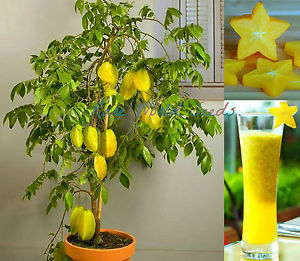
\includegraphics[width= 0.45\linewidth]{carambTree.jpeg} \hfill 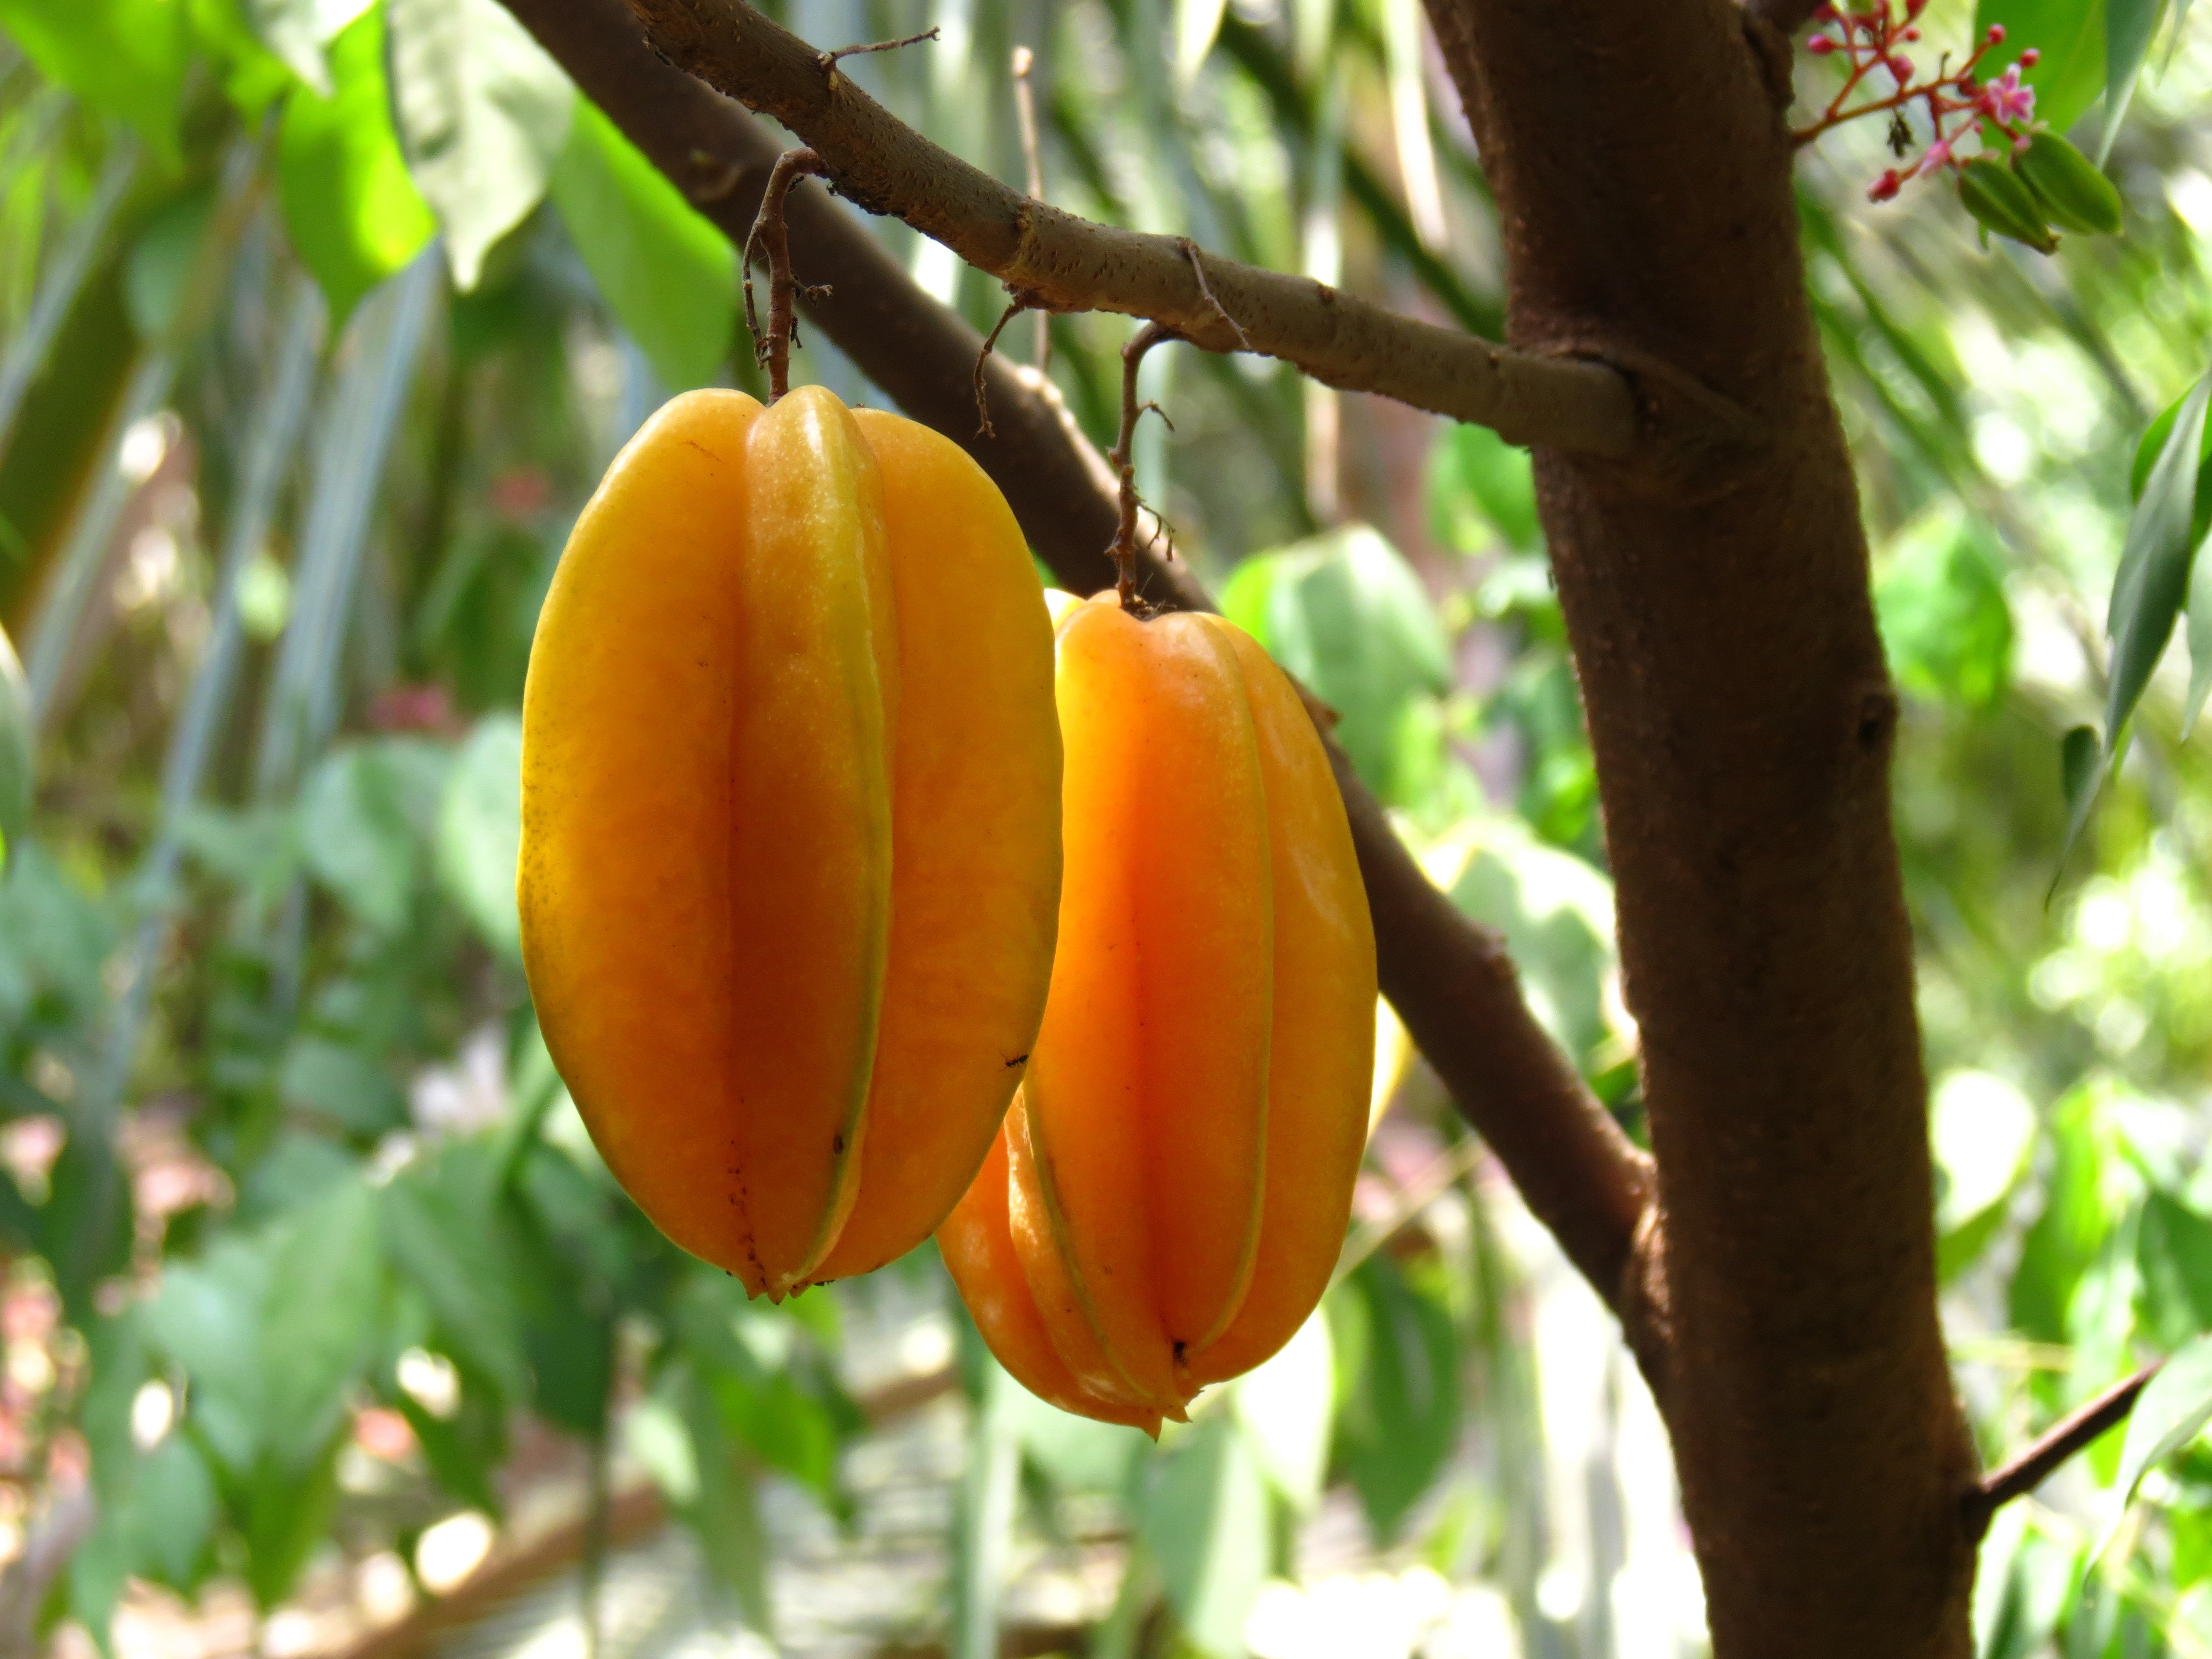
\includegraphics[width= 0.45\linewidth]{carambFruit.jpg}

\end{frame}

\subsection{Nutation movement}
\begin{frame}{What is nutation ?}
\begin{center}
\movie[width=9cm, height=6cm, poster]{}{nutation.webm}
\end{center}


\end{frame}

\subsection{Scientific question}
\begin{frame}{Scientific question}

\vfill
$\bullet$ Does the nutation synchronizes with the day/night cycle ?
\vfill
$\bullet$ Is the nutation influenced by the temperature ?
\vfill
$\bullet$ Is the nutation influenced by the light cycle ?
\vfill

\end{frame}

\section{Regulation system}
\subsection{Arduino system}

\begin{frame}{The Arduino system}
\begin{center}
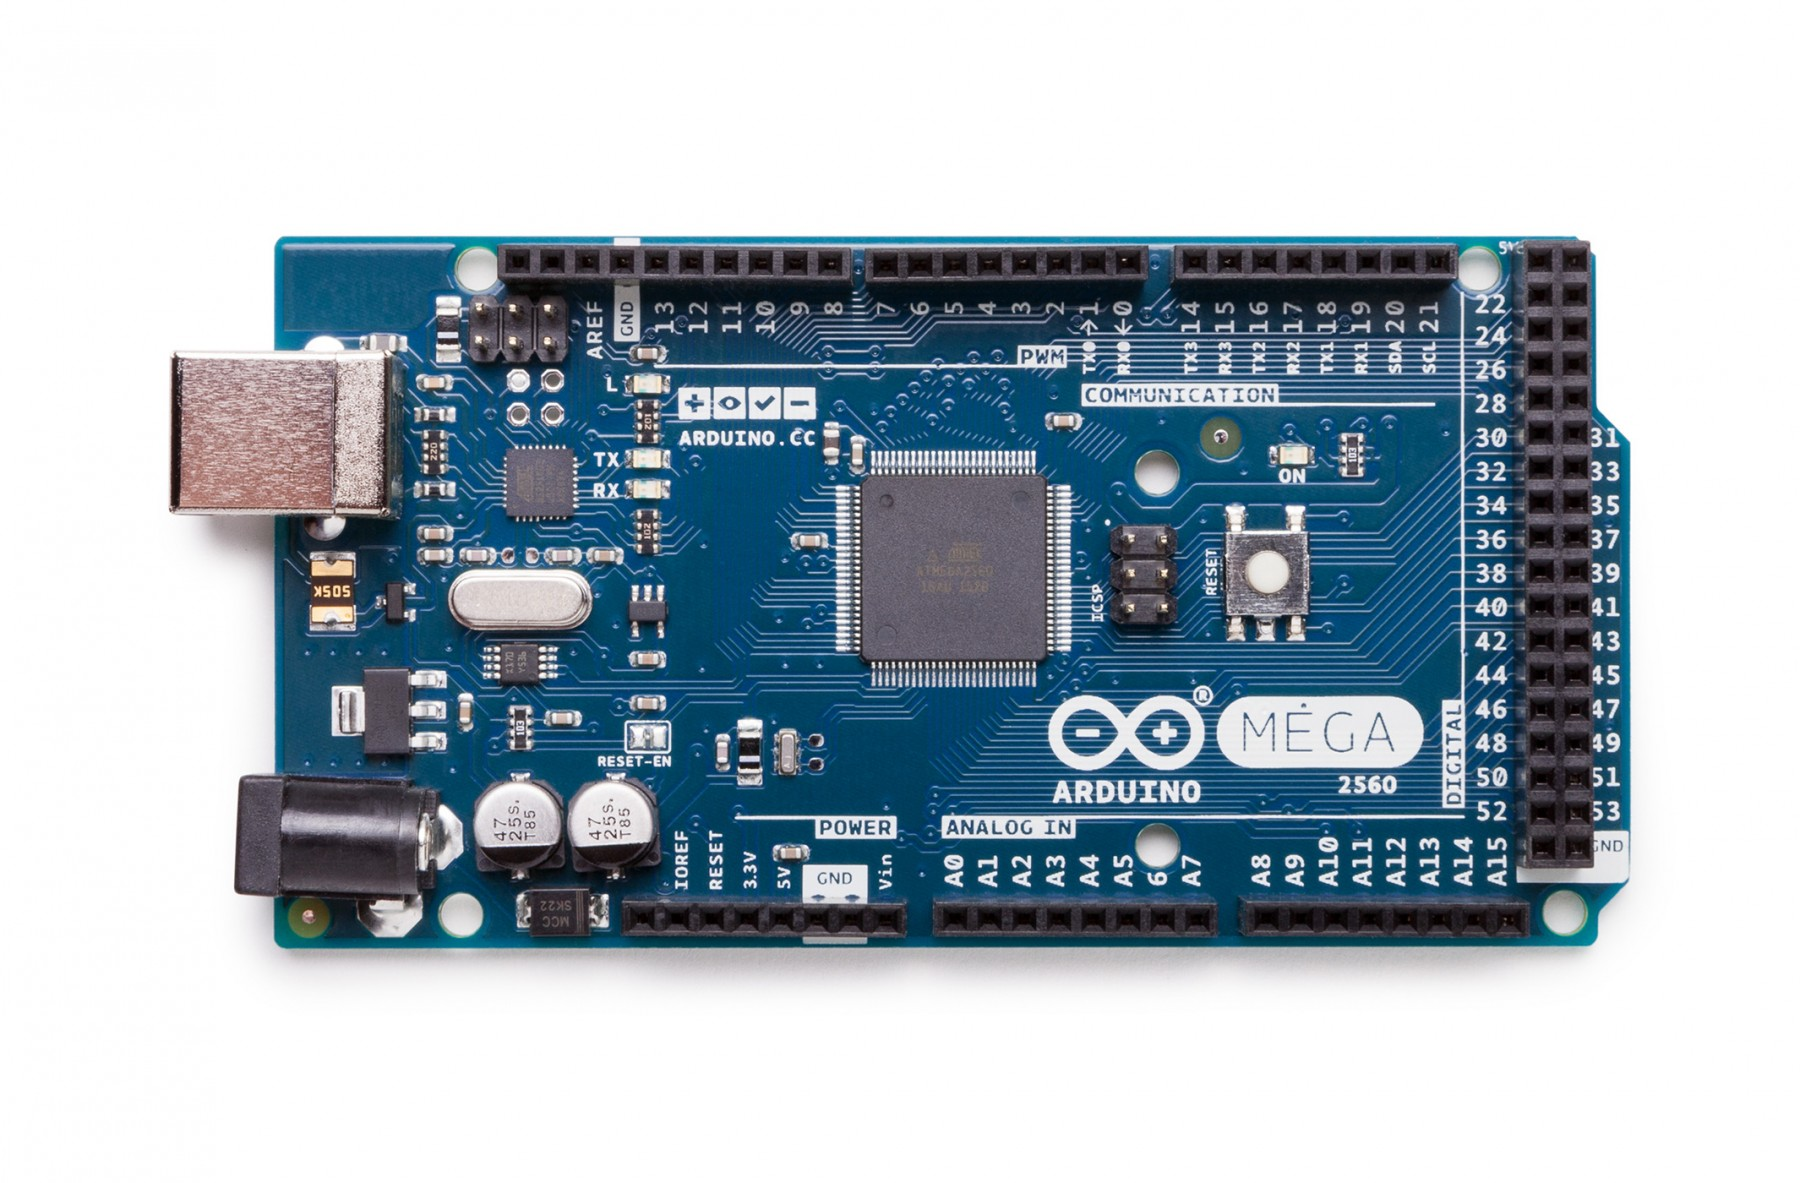
\includegraphics[width=0.3\linewidth]{arduino.jpg} \hspace{1cm} 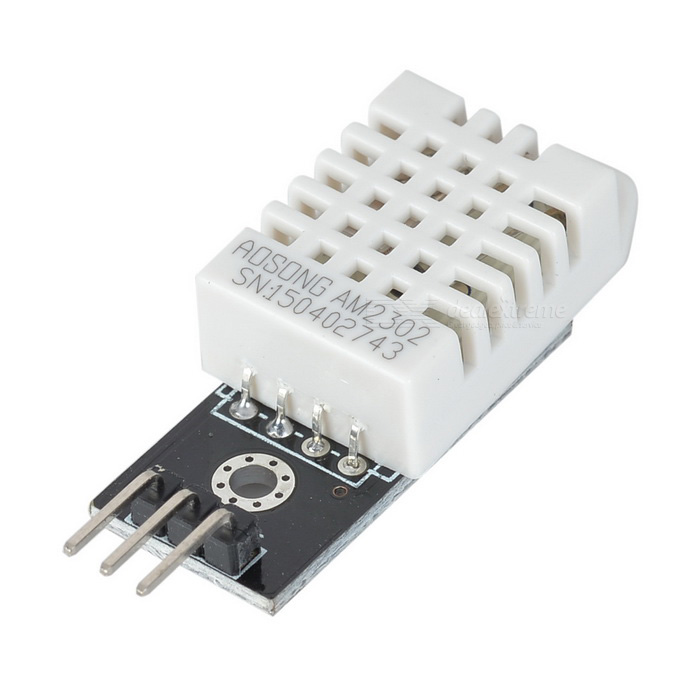
\includegraphics[width=0.15\linewidth]{dht22.jpg}
\[ \downarrow \]
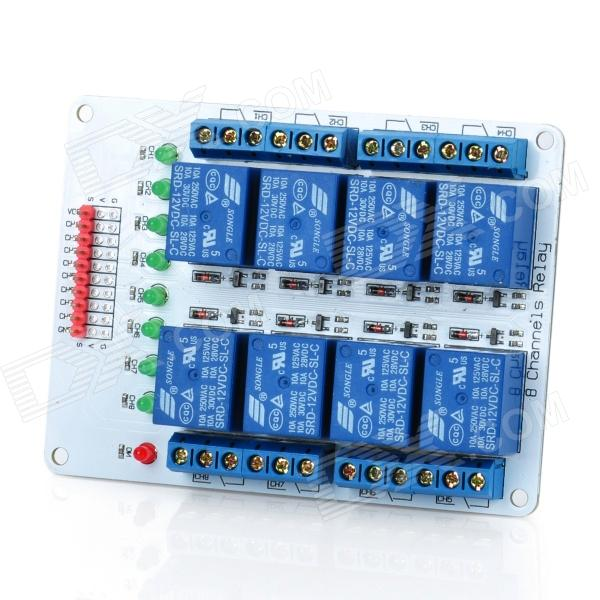
\includegraphics[width = 0.2 \linewidth]{relays.jpg} \hspace{2cm}
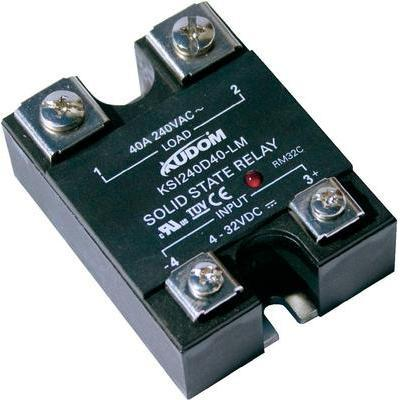
\includegraphics[width = 0.2\linewidth]{relayStat.jpg}
\end{center}
\end{frame}

\begin{frame}{My system}
\begin{center}
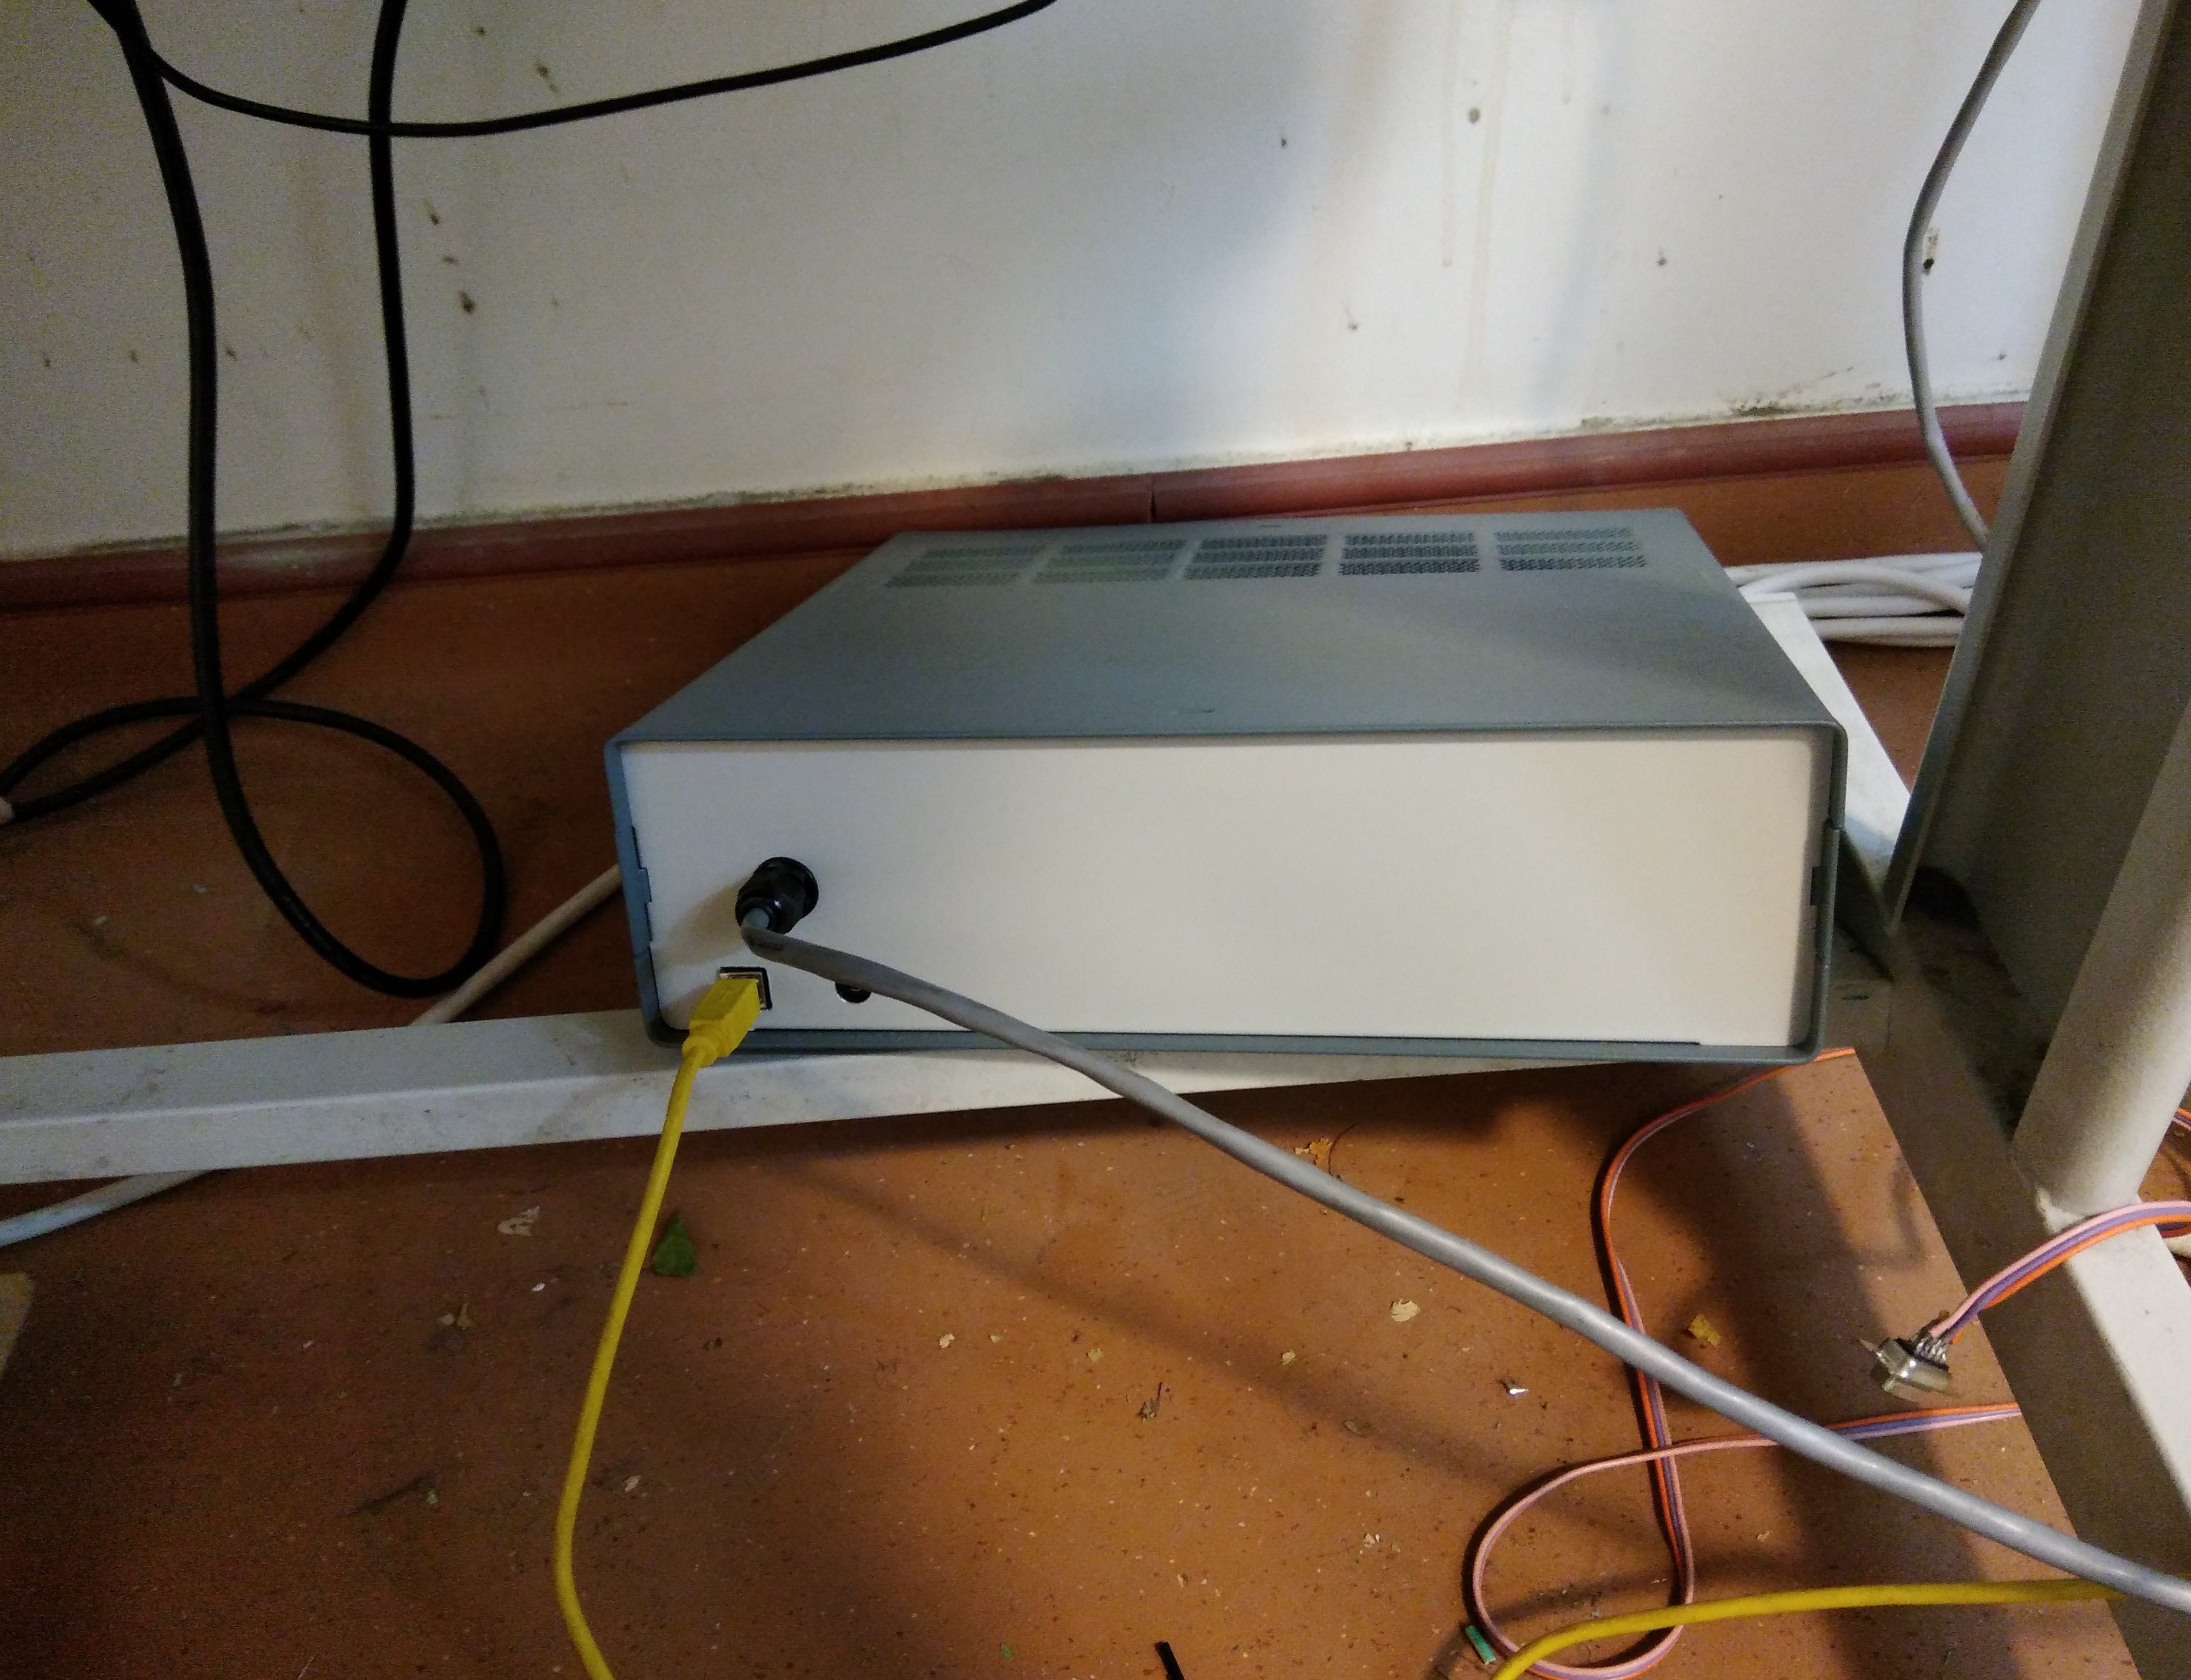
\includegraphics[width=0.6\linewidth]{boitier.jpg}
\end{center}
\end{frame}

\subsection{Peripherals}

\begin{frame}{Devices}
\begin{center}
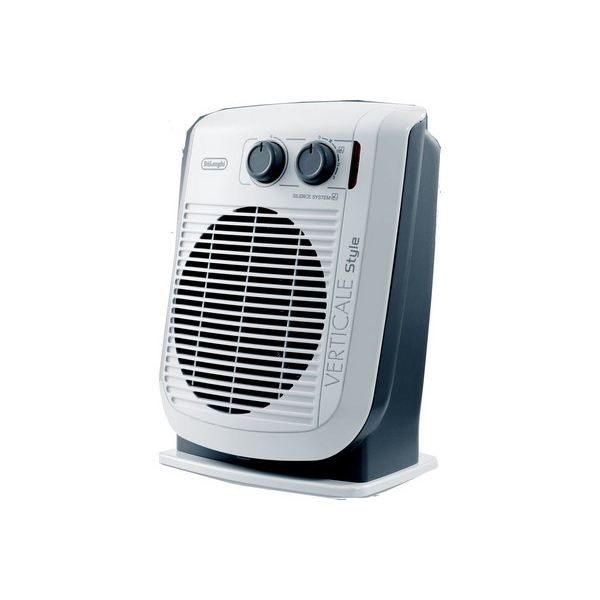
\includegraphics[width = 0.3\linewidth]{chauffage.jpg} \hspace{1cm} 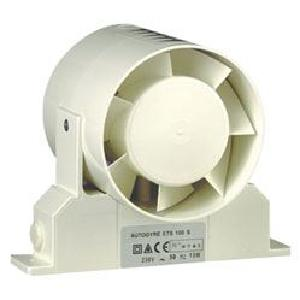
\includegraphics[width = 0.3\linewidth]{ventil.jpg} ~\\

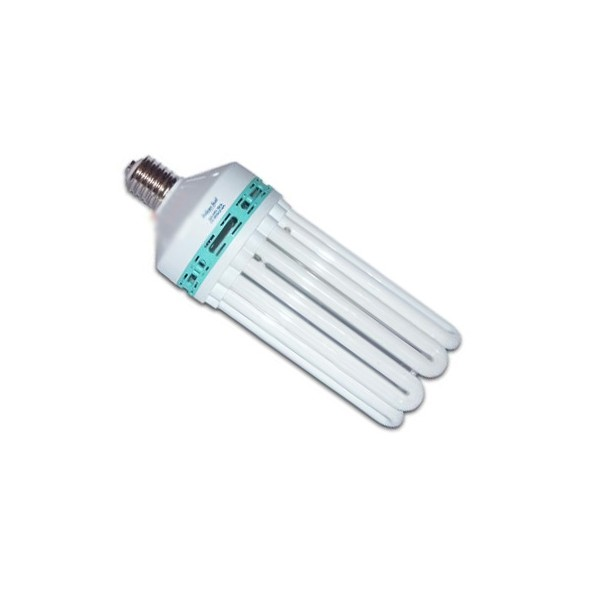
\includegraphics[width = 0.3\linewidth]{lampe.jpg} \hspace{1cm} 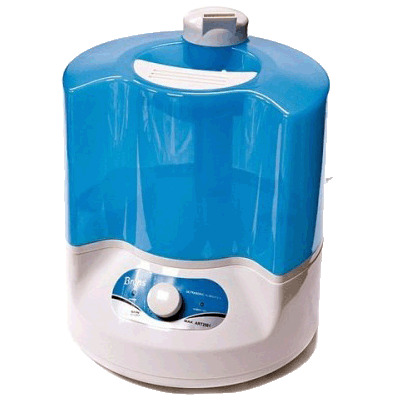
\includegraphics[width = 0.3\linewidth]{humidificateur.jpg}
\end{center}

\end{frame}

\section{Analysis}
\subsection{Getting the trajectory}
\begin{frame}{Picture setup}
\begin{center}
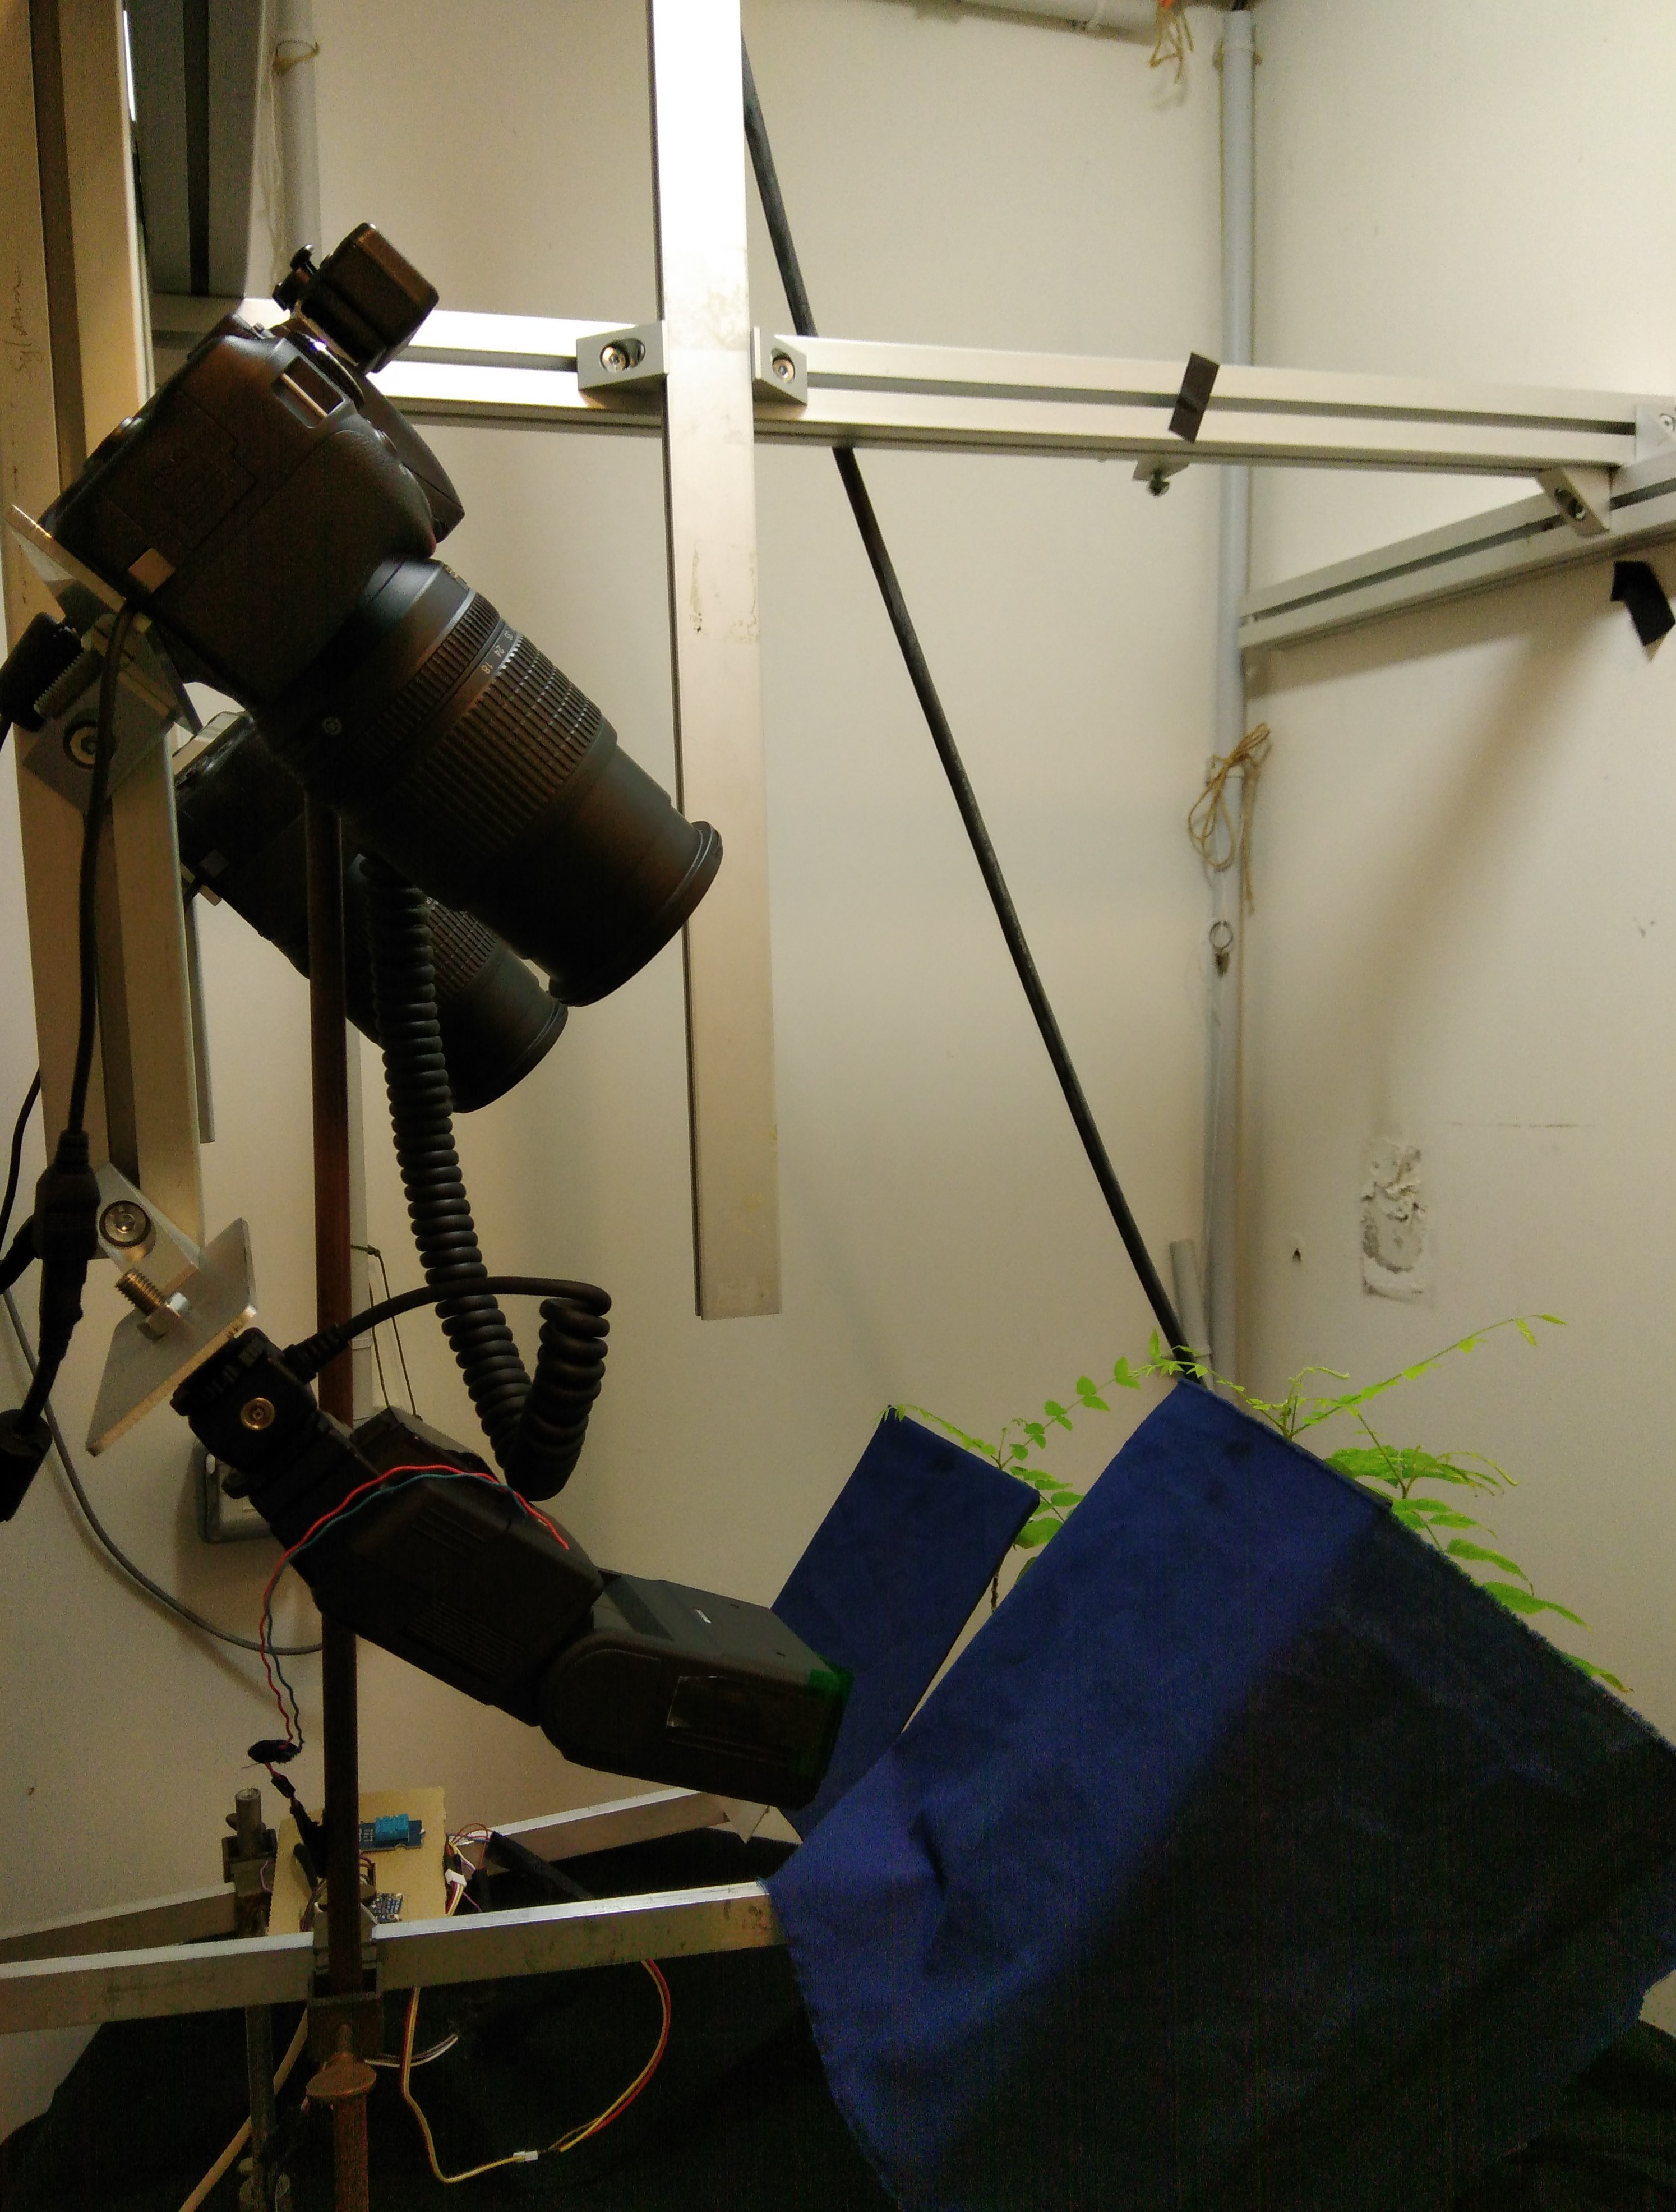
\includegraphics[width = 0.2\linewidth]{appareils.jpg} \hspace{1cm} \includegraphics[width = 0.4\linewidth]{imKymo.jpg} ~\\

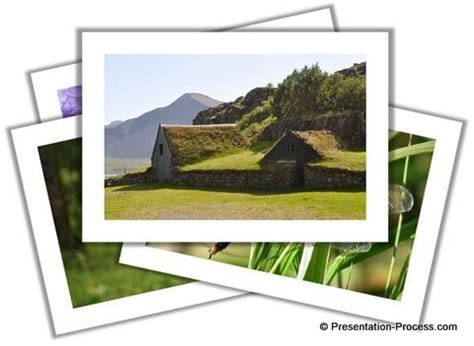
\includegraphics[width = 0.3\linewidth]{picStack.jpg} \hspace{1cm} 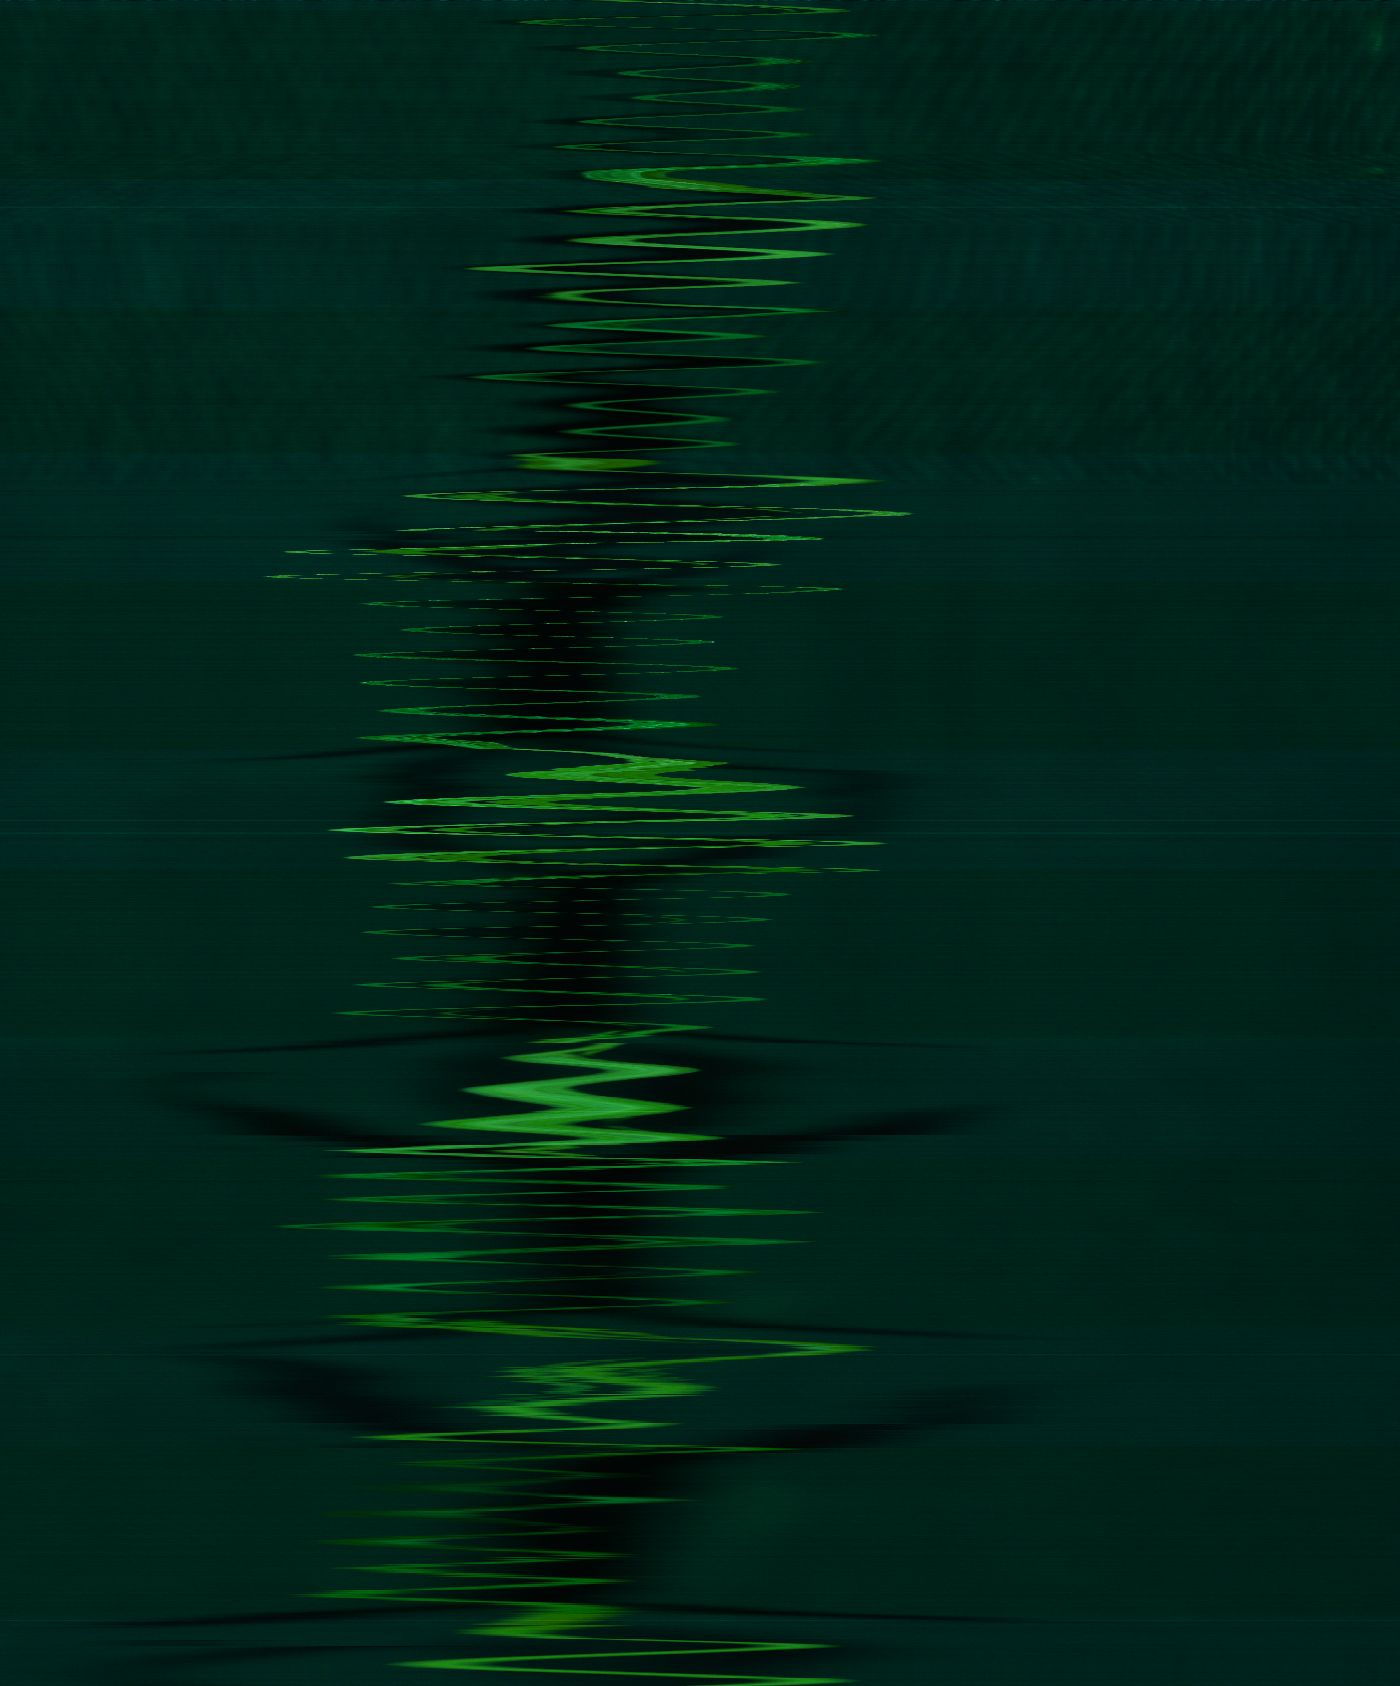
\includegraphics[width = 0.3\linewidth]{kymo.png}

\end{center}

\end{frame}

\begin{frame}{The trajectory}
\begin{center}
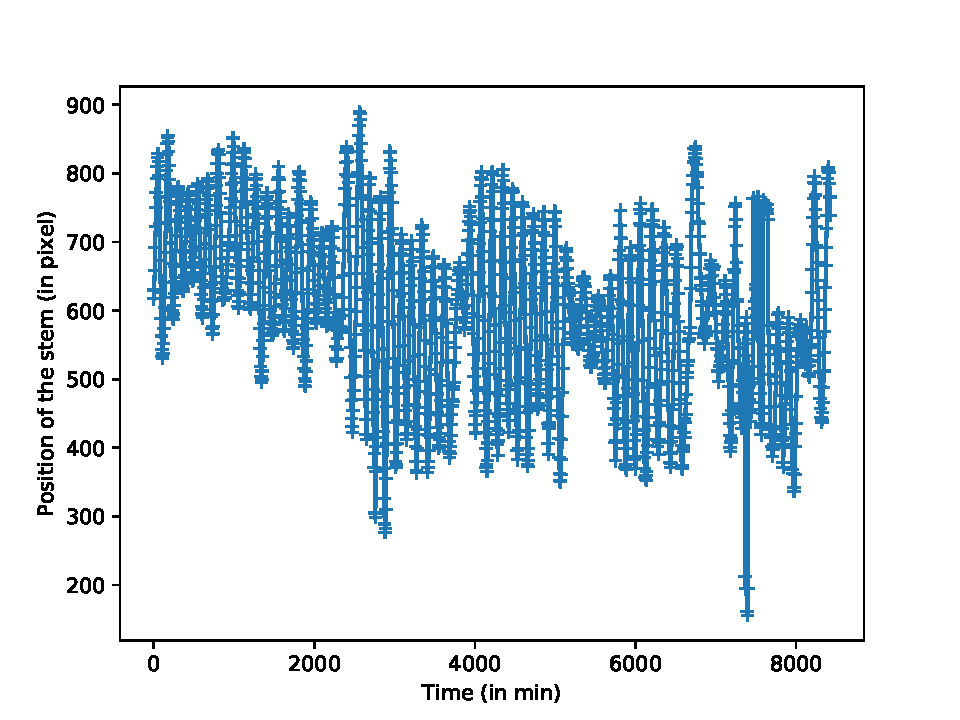
\includegraphics[width = 0.75\linewidth]{traj.pdf} %\hspace{1cm} \includegraphics[width = 0.4\linewidth]{trajScaled.pdf}
\end{center}

\end{frame}

\subsection{Correcting the deviation}
\begin{frame}{Correction with linear regression}
\begin{multicols}{2}
\begin{figure}
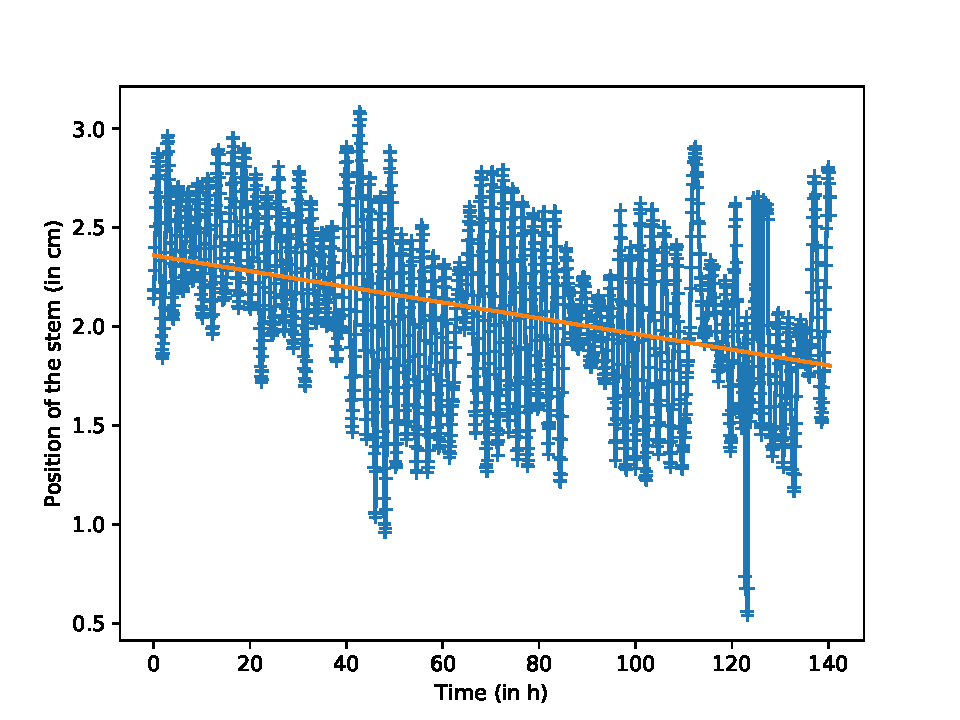
\includegraphics[width = \linewidth]{trajScaledRaw.pdf}~\\
Raw trajectory with the linear regression
\end{figure}
\begin{figure}
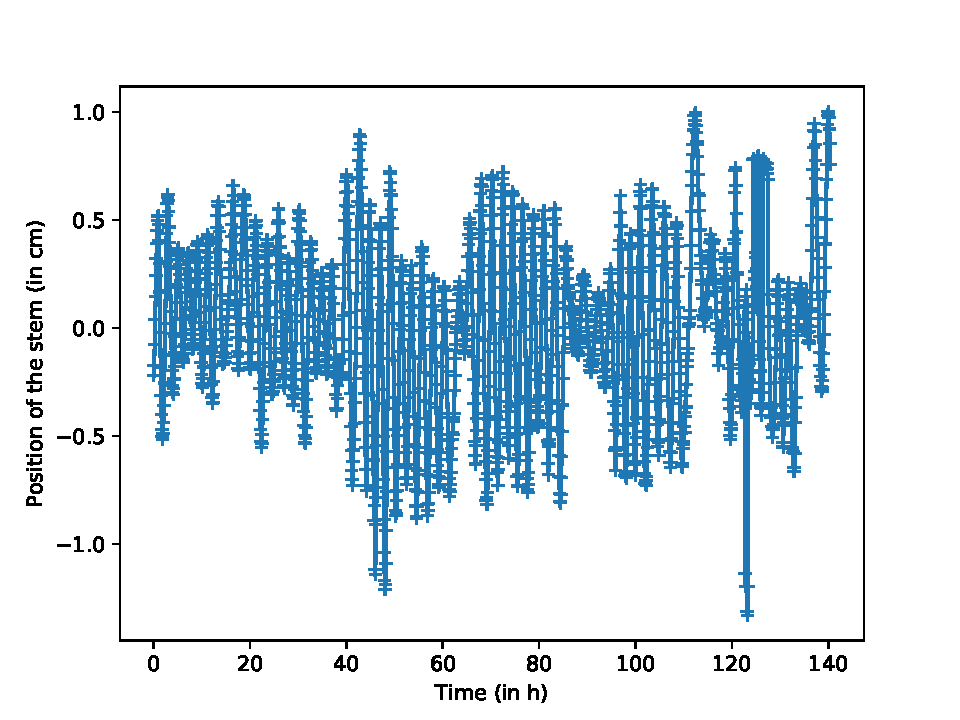
\includegraphics[width = \linewidth]{trajScaledCorr.pdf}~\\
Corrected trajectory
\end{figure}
\end{multicols}
\end{frame}

\subsection{Wavelet analysis}
\begin{frame}{Presentation of the wavelet analysis}

\begin{figure}

\includegraphics[width = 0.75\linewidth]{powergraph.pdf}~\\
Powergraph of the wavelet analysis
\end{figure}

\end{frame}

\begin{frame}{Result of the Wavelet Analysis}
\begin{multicols}{2}
\begin{figure}
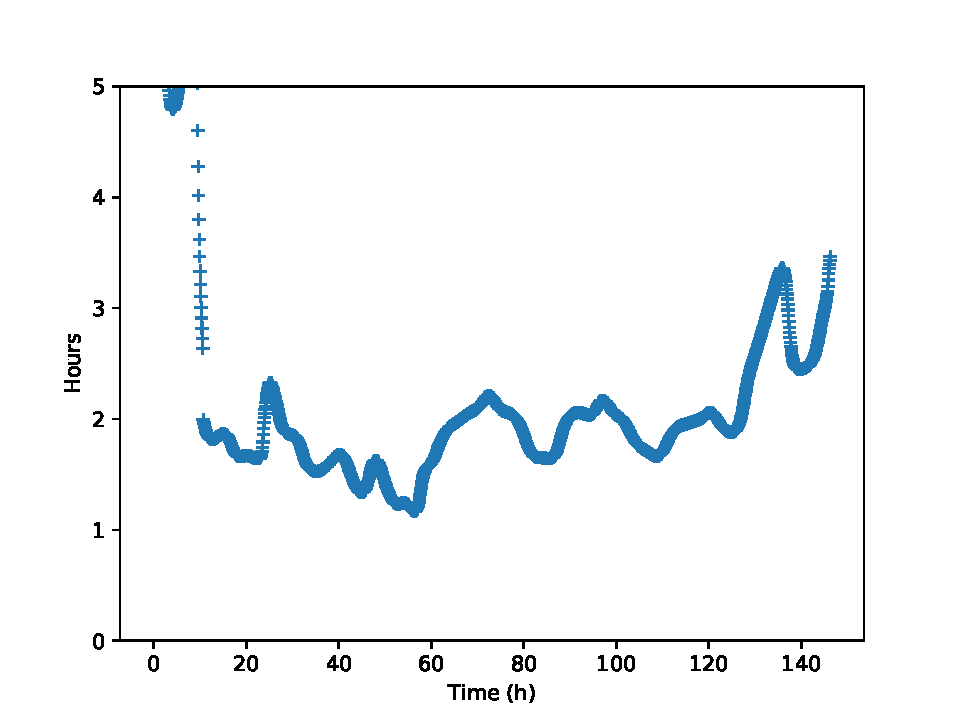
\includegraphics[width = \linewidth]{period.pdf}~\\
Period of the nutation
\end{figure}
\begin{figure}
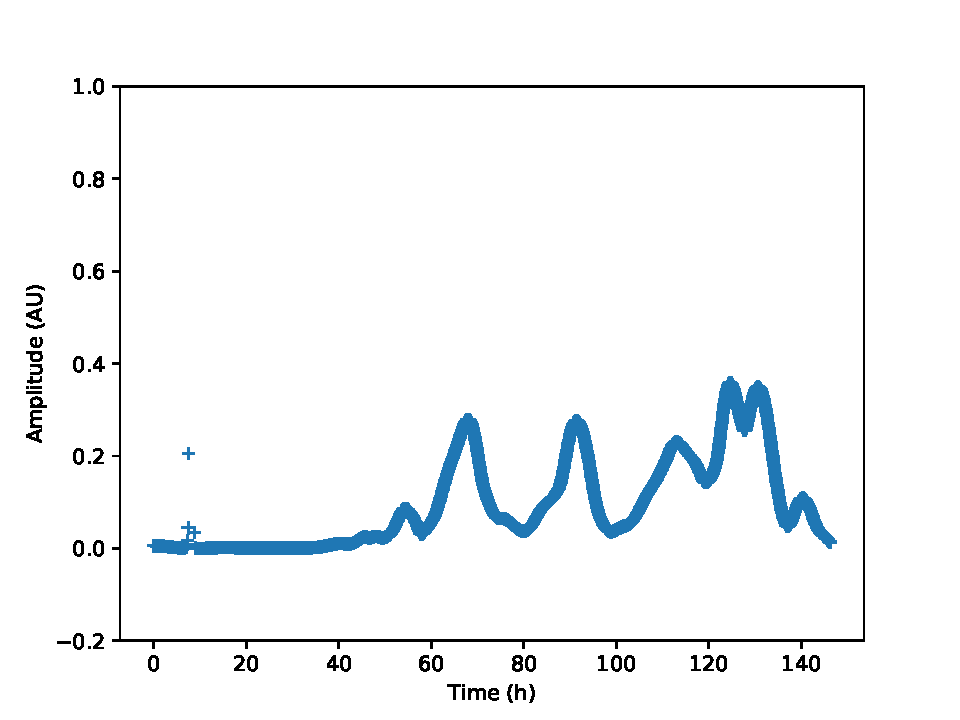
\includegraphics[width = \linewidth]{ampl.pdf}~\\
Amplitude of the nutation
\end{figure}
\end{multicols}
\end{frame}

\section{Results}
\subsection{at \SI{24}{\celsius}}
\begin{frame}{\SI{24}{\celsius}}
\begin{multicols}{2}
\begin{figure}
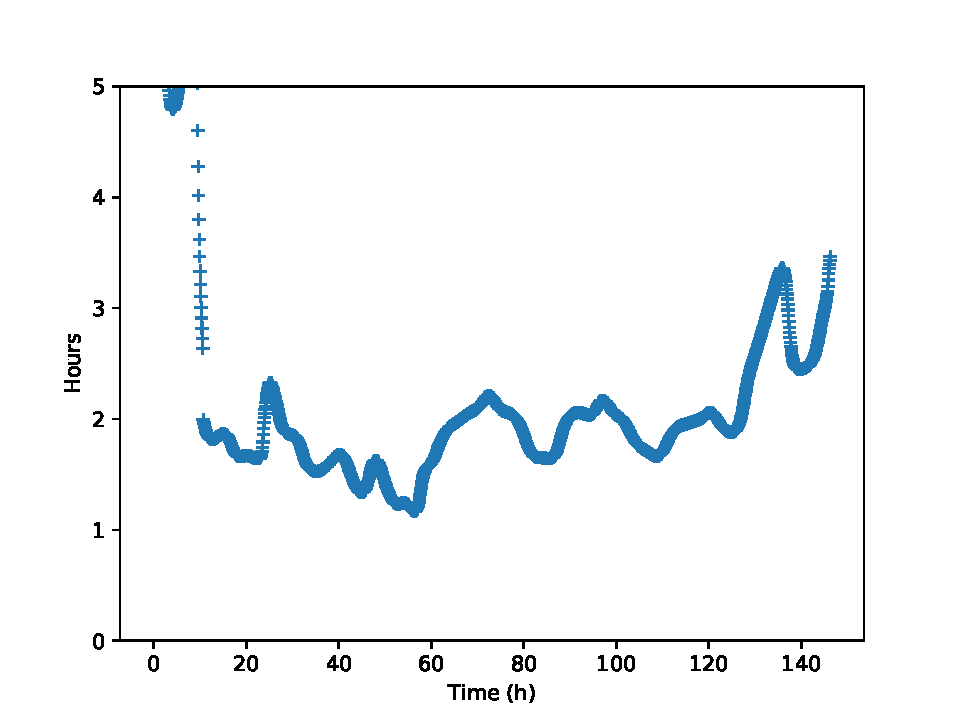
\includegraphics[width = \linewidth]{period.pdf}~\\
Period of the nutation at \SI{24}{\celsius}
\end{figure}
\begin{figure}
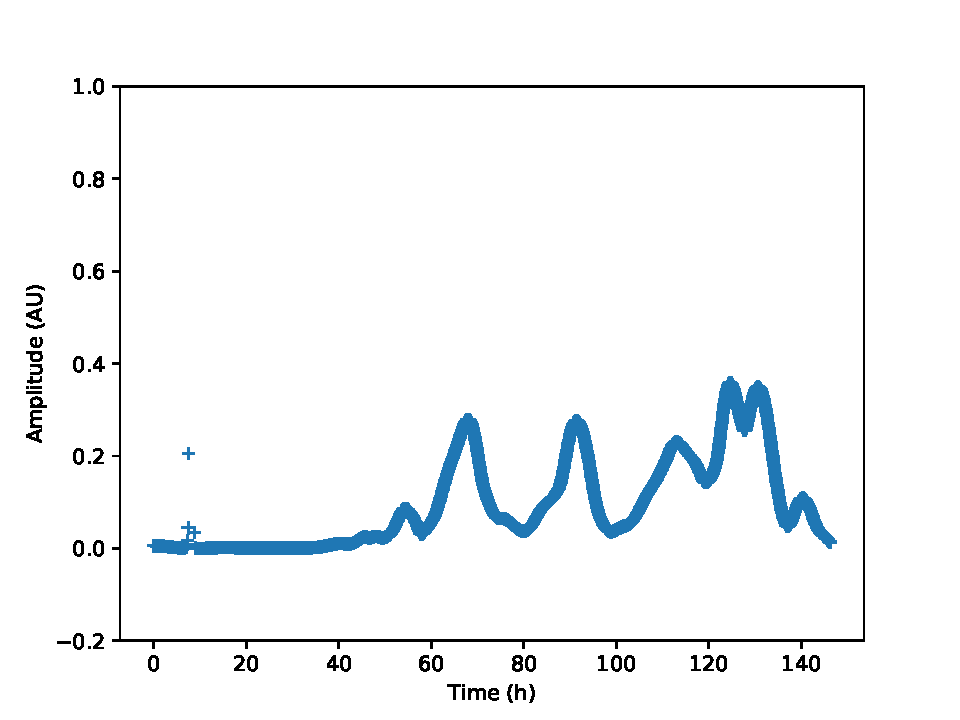
\includegraphics[width = \linewidth]{ampl.pdf}~\\
Amplitude of the nutation at \SI{24}{\celsius}
\end{figure}
\end{multicols}
\end{frame}

\subsection{at \SI{22}{\celsius}}
\begin{frame}{\SI{22}{\celsius}}

\begin{multicols}{2}
\begin{figure}
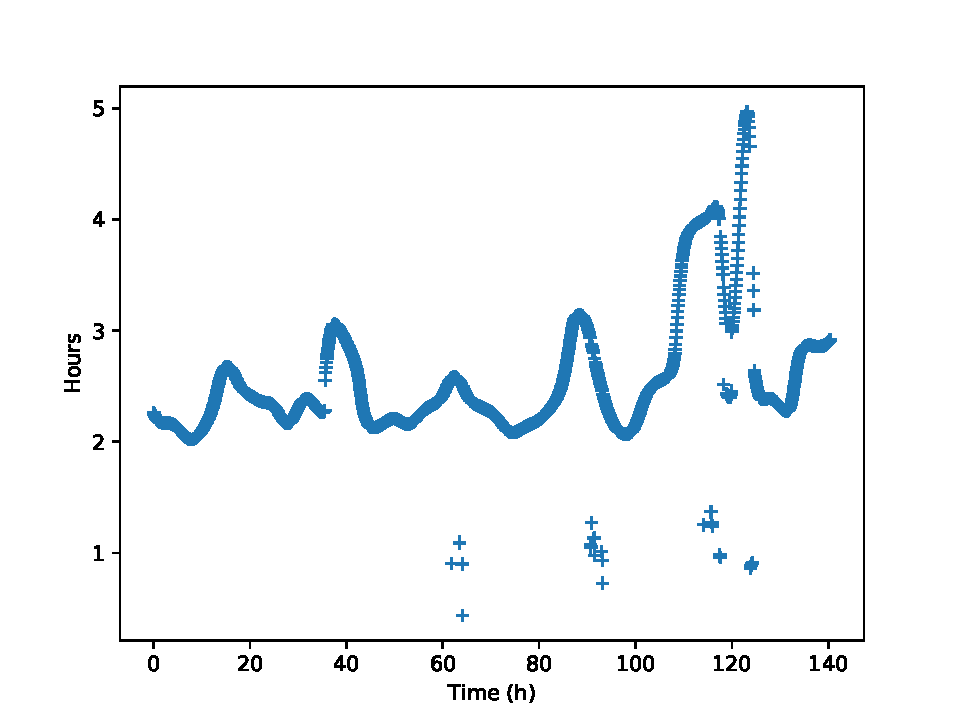
\includegraphics[width = \linewidth]{period22.pdf}~\\
Period of the nutation at \SI{22}{\celsius}
\end{figure}
\begin{figure}
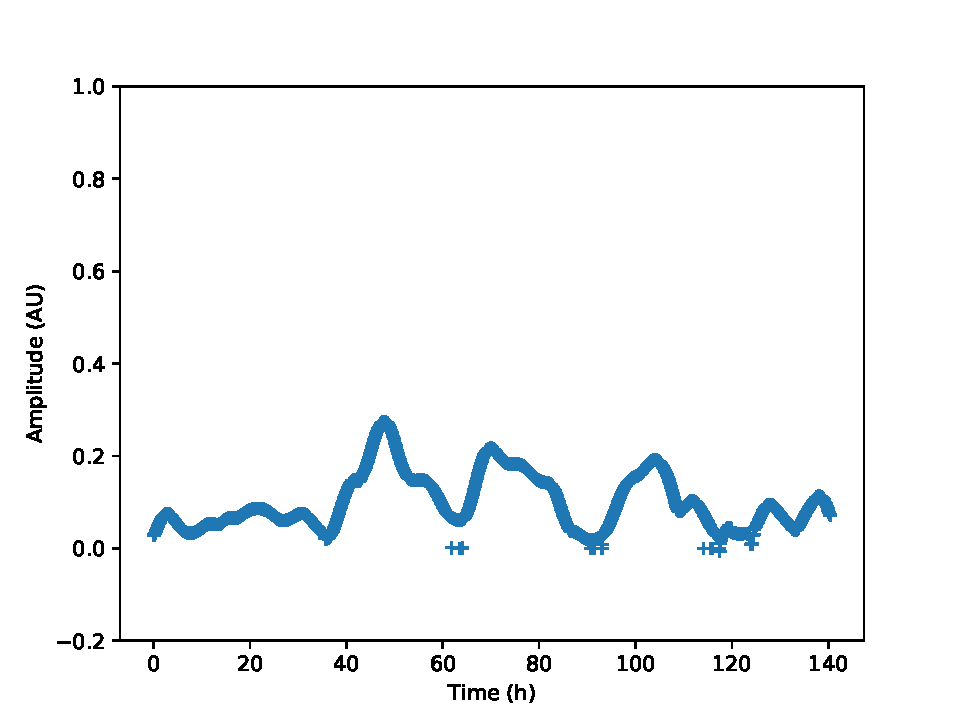
\includegraphics[width = \linewidth]{ampl22.pdf}~\\
Amplitude of the nutation at \SI{22}{\celsius}
\end{figure}
\end{multicols}

\end{frame}

\subsection{at \SI{28}{\celsius}}
\begin{frame}{\SI{28}{\celsius}}
\begin{multicols}{2}
\begin{figure}
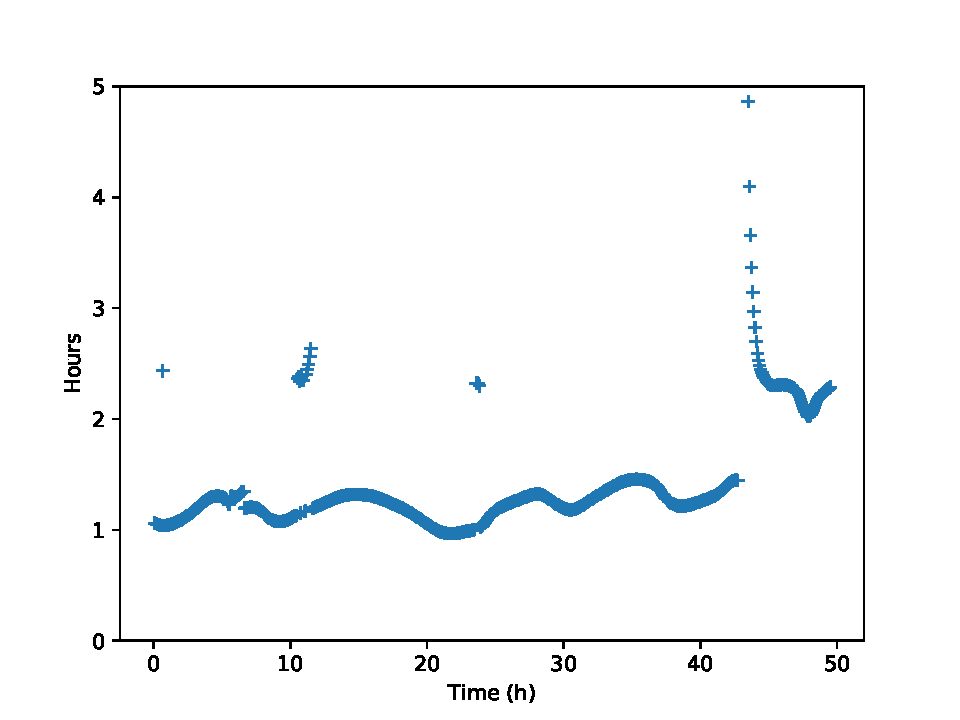
\includegraphics[width = \linewidth]{period28.pdf}~\\
Period of the nutation at \SI{28}{\celsius}
\end{figure}
\begin{figure}
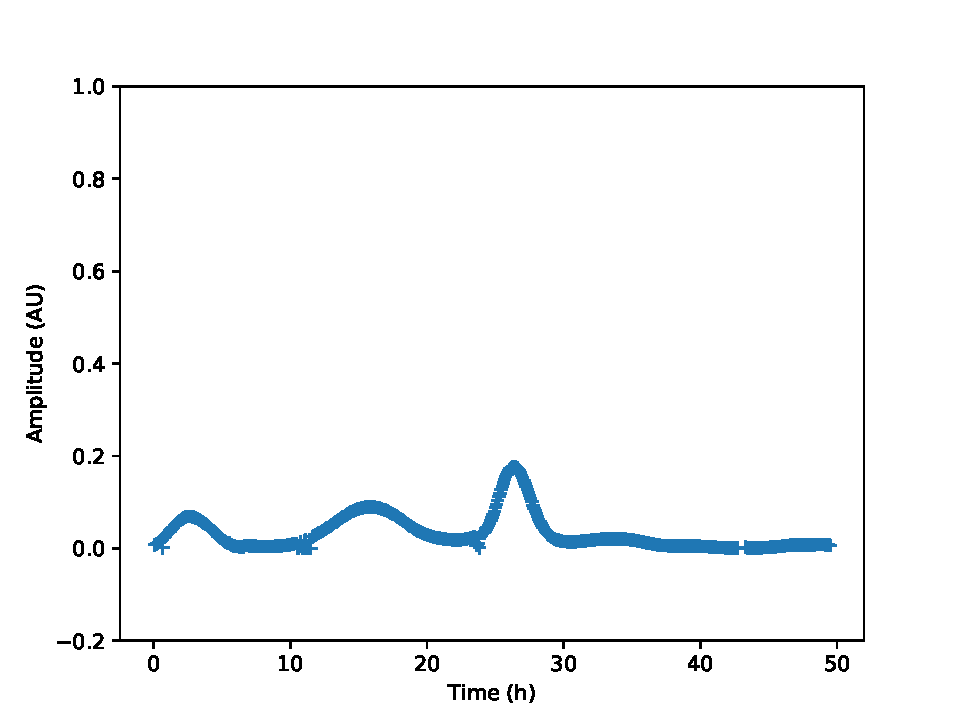
\includegraphics[width = \linewidth]{ampl28.pdf}~\\
Amplitude of the nutation at \SI{28}{\celsius}
\end{figure}
\end{multicols}
\end{frame}

\section{Conclusion}
%\subsection{Conclusion}
\begin{frame}{Conclusion}
\vfill
\[ \text{Period of nutation } \searrow \text{~~~~~~~~when Temperature } \nearrow \]
\vfill
\[  \text{Amplitude of nutation} \searrow \text{~~~~~~~~when Temperature } \nearrow\]
\vfill
\hrule
\vfill
$\bullet$ Do more replicate to observe more general behaviour
\vfill
$\bullet$ Try with different photoperiods, cycles of temperature...

\end{frame}

\section{Thanks}
\begin{frame}{Thanks}
\begin{center}
\vfill
Thanks to my supervisor Julien \textsc{Derr},
\vfill
to Stéphane for his ideas,
\vfill
to the PhDs of the lab for their help
\vfill
and you for your attention !
\vfill
%
\includegraphics{caramBye.jpg}
\end{center}
\end{frame}



\end{document}